\documentclass[finnish,colorlinks,headings=normal,parskip=half,footsepline]{scrartcl}

\usepackage[utf8]{inputenc}
\usepackage[T1]{fontenc}
\usepackage{libertine,babel,setspace,ragged2e,scrlayer-scrpage,lastpage,geometry,calc,graphicx,wrapfig}
\usepackage[activate=false,stretch=0,letterspace=120]{microtype}
\usepackage{hyperref}

\RaggedRight
\frenchspacing
\setstretch{1.04}
\setkomafont{pageheadfoot}{\scriptsize\sffamily}
\setkomafont{pagenumber}{\scriptsize\sffamily}
\addtokomafont{disposition}{\rmfamily}
\urlstyle{same}
\clearpairofpagestyles
\lofoot*{\lsstyle\MakeUppercase{J.~Suomalainen: insta}}
\rofoot*{\lsstyle SIVU~\pagemark/\pageref{LastPage}}
\newcommand*\GetTextWidth[3][\normalfont]{{#1%
		\settowidth{#2}{abcdefghijklmnopqrstuvwxyz}%
		\setlength{#2}{0.03193#2}%
		\addtolength{#2}{0.44961pt}%
		\setlength{#2}{#3#2}%
		\global#2=#2}}
\newlength\bringhurstwdt
\GetTextWidth{\bringhurstwdt}{70}
\geometry{top=1.5in,bottom=1.75in,textwidth=\bringhurstwdt}
\addtolength{\footskip}{-22pt}

\begin{document}
Janne Suomalainen\\\textsf{insta} (0.9)\\Web"-palvelinohjelmointi Java "=kurssin harjoitustyö\\\today

\section{Sovellus}
Sovellus löytyy osoitteesta \url{https://evening-island-18993.herokuapp.com}. Sovelluksen lähdekoodi löytyy \href{https://github.com/suomja1/insta}{GitHubista} ja sen testaus (versiossa 0.9 ei ole implementoitu yhtään testiä) on automatisoitu \href{https://travis-ci.org/suomja1/insta}{Travis-palvelun} avulla.

\textsf{insta} on pelkistetty kuvapalvelu (vertaa \href{https://www.instagram.com}{Instagram}), jossa käyttäjä pystyy lisäämään, selaamaan sekä kommentoimaan kuvia. Kuvien selaamisen helpottamiseksi kuviin voi lisätä erilaisia tunnisteita (vertaa \emph{hashtag}).

Erilliset tuotanto- ja testausprofiilit sujuvoittavat sovelluksen kehittämistä. \textsf{insta}ssa profiilit on toteutettu erillisillä konfiguraatiotiedostoilla ja Springin tarjoamalla Profile"-annotaatiolla. Käytettävä profiili valitaan sovelluksen main"-luokassa SpringApplication"-luokan setAdditionalProfiles"-metodilla.

\begin{wrapfigure}[15]{r}{.5\linewidth-.5\columnsep}
\vspace*{-\intextsep}
\centering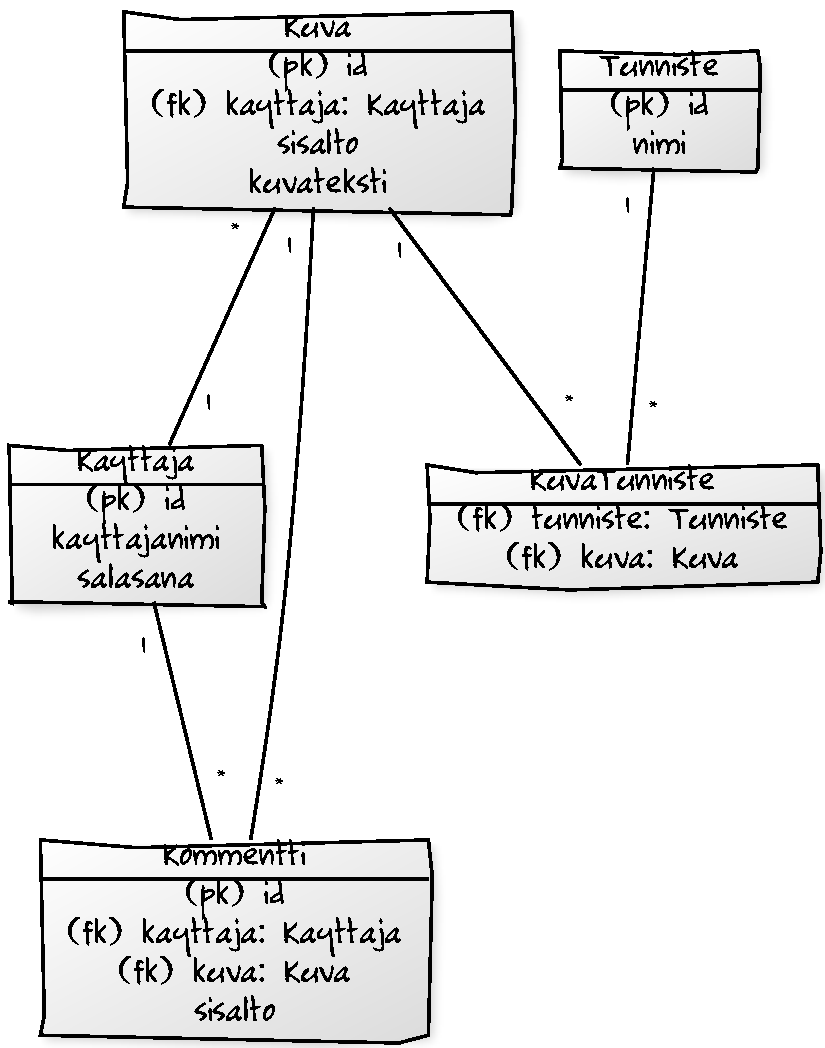
\includegraphics[width=\linewidth]{6424b8c7}
\caption{Tietokantakaavio.}\label{fig:tk}
\end{wrapfigure}

Sovellus käyttää tietokantaa, jossa on yhteensä viisi taulua. Yksi näistä on liitostaulu. Testausprofiilissa käytetään H2 Database "-tietokantaa, joka ladataan muistiin aina sovelluksen käynnistyessä. Tuotantoprofiilissa käytetään Herokun tarjoamaa Postgres"-tietokantaa. Tietokantakaavio on esitetty kuvassa~\ref{fig:tk}.

\section{Keskeisiä käyttötapauksia}
Uusi käyttäjä pystyy luomaan tunnuksen sovelluksen kirjautumissivulla syöttämällä Luo käyttäjä "=otsakkeen alla oleviin kenttiin käyttäjänimen ja salasanan. Käyttäjänimi on uniikki, 4--30 merkkiä pitkä merkkijono, salasana yli 6 merkkiä. Merkkien pituus on validoitu -- tosin englanninkielisin virheviestein.

Käyttäjä pystyy kirjautumaan sovellukseen syöttämällä Kirjaudu sisään "=otsakkeen alla oleviin kenttiin käyttäjänimen ja salasanan. Kirjautumisen epäonnistuessa annetaan selkokielinen virheviesti. Sisäänkirjauduttuaan käyttäjä pystyy kirjautumaan ulos sivun oikeassa ylälaidassa olevasta Kirjaudu ulos "=painikkeesta.

Uuden kuvan lisääminen käy kotisivun alareunassa olevalla lomakkeella. Lomakkeella valitaan kuvatiedosto, kuvan kuvateksti ja tunnisteet. Jälkimmäiset näistä ovat vapaaehtoisia. Kuvatiedostolla on kokorajoitus. Tunnisteet syötetään pilkuin erotettuna listana. Latauksen onnistuessa kuva piennennetään ja lisätään tietokantaan kuvateksteineen ja tunnisteineen.

Käyttäjä pystyy selata kuvia kolmella eri tavalla: käyttäjittäin, tunnisteittain ja yksittäin. Käyttäjä- ja tunnistekohtaisilla sivuilla kuvista kerrotaan käyttäjän tai tunnisteen lisäksi kuvan kuvateksti, kuvan lisääjä ja kommenttien lukumäärä. Kuvakohtaisella sivulla listataan kaikki kuvan tunnisteet ja kommentit.

Kuvan kommentointi tapahtuu kuvakohtaisen sivun alareunassa olevalla lomakkeella. Kommentti tallentuu aina kirjautuneen käyttäjän nimellä kuvan alle.

navigointi

\section{Jatkokehitys}
Sovellukselle pitää kirjoittaa kattavat yksikkö-, integraatio- ja järjestelmätestit.

Yritettäessä luoda uutta käyttäjää, jolla on sama käyttäjänimi jo olemassa olevan käyttäjän kanssa, antaa sovellus automaattisen virheviestin (500). Tämä ei ole kaunista luettavaa. Käyttäjänimen uniikkius tulisi validoida ennen yritystä kirjoittaa tietokantaan. Lisäksi sovellus ei ilmoita käyttäjälle, jos käyttäjän luominen onnistuu.

Lisää kuva -lomaketta ei ole validoitu. Kuvateksti- ja tunniste-kenttien kohdalla tämä ei ole välttämätöntä, mutta tiedostotyypin ja "=koon tarkastaminen olisi oleellista.

Tietokantatauluihin voisi lisätä ajankohta-attribuutin, jolloin esimerkiksi kommentit voitaisiin järjestään niiden lisäämisajankohdan mukaan.

roolit

virheviestit
\end{document}